\newpage
\section{Technologies}

\subsection{Wave}

In the making of this work every extension has been developed and tested under two varieties of Wave: Wave In A Box and Kune. Kune nowadays has much of it's code forked from the Wave In A Box repository, but adding more functionality around it. Gadgets and apps are built into the core of Wave, and as such Kune inherits all their capabilities, making gadgets and robots comparible with both technologies.

\begin{figure}[h]
  \center
    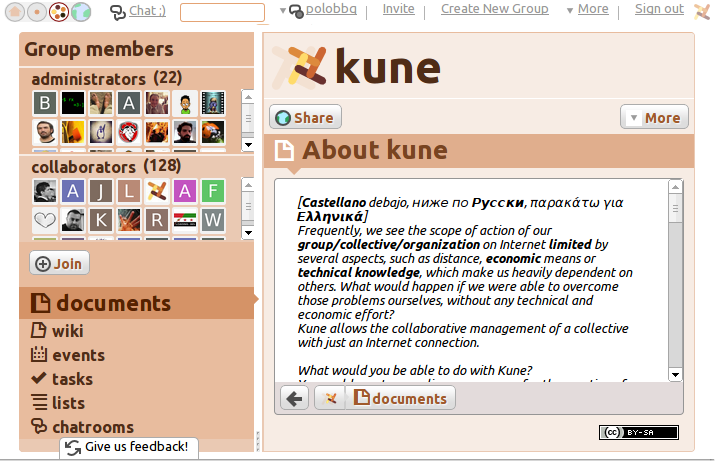
\includegraphics[keepaspectratio, scale=0.4]{Media/Captures/Wave/Kune_Groups.png}
  \caption{Kune Groups}
  \label{fig:kune_groups}
\end{figure}

The main technical feature that characterizes Wave is the Wave Federation Protocol \cite{ref:wave_federated_protocol}, that handles all of the communication happenning between users. It is an esxtension of the Extensible Messaging and Presence Protocol \cite{ref:xmpp}. Participants send delta changes on the content, and those deltas are distributed through the rest of the participants, guaranteeing that the end result is the same for everyone \cite{ref:federating_websites_google_wave}. Gadgets and robots will work under this environment, interacting with the Wave protocol.


\subsection{GWT}

Google Web Toolkit GWT is a set of tools that allows web developers to code in Java and from that java-compliant code, generate Asynchronous JavaScript and XML (AJAX) code to make front-end applications. The GWT framework focuses on efficiency and cross-browser compatibility, generating and then serving different AJAX code for every browser and locale combination, so the elements are rendered as they should in each browser, even though they behave differently. GWT provides the developer with all the common web controls, allows RPC invokations, browser history management, unit testing, and native JavaScript calls, among other features.

\begin{figure}[h]
  \center
    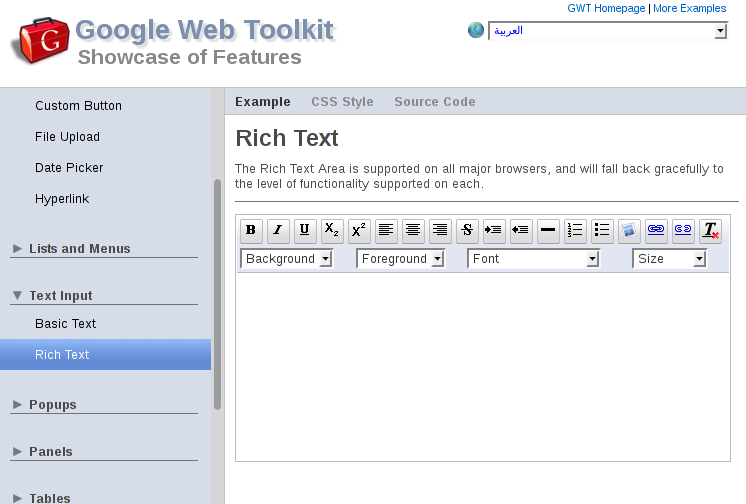
\includegraphics[keepaspectratio, scale=0.4]{Media/Captures/GWT/gwt_showcase.png}
  \caption{GWT Showcase}
  \label{fig:gwt_showcase}
\end{figure}

GWT has a development mode, where the Java code is not compiled to JavaScript, but instead it is ran in native Java and simulates the JavaScript components that will be used later. The development mode also allows a Java debugger to attach to GWT and debug the application locally. 


\subsection{Gadgets API}

The Gadgets API is made by Google to embed third party applications inside various Google products. They implemented it in wave as Wave Gadgets API, to have access to the specific features of Wave. These applications are HTML and JavaScript, with all their possibilities, and access specific features that the server can offer.

This is a Java API, and it needs to be compiled with the GWT compiler in order to be able to link to the gadgets. Apart from being able to use all GWT components, this API lets the developer communicate with Wave, and that means mainly altering the state and responding to state changes. The state contains the participants, and the content, among other information. 


\subsection{Robots API}

It is an API with client libraries for Java an Python, both of them implementing the same set of features. The original intention was that robots could act in Wave in exactly the same places and same ways as human participants could. In practice, not all interactions are implemented for robots. A robot can be added to a Wave, can edit text, add participants, publish new Wavelets, and access the contents of all of them, as well as responding to events about changes in the document or participants.


\subsection{Other}

\begin{itemize}
  \item As IDE Eclipse 3.8 has been used for developing the gadgets as well as the robot.
  \item OpenJDK has been used as JDK
  \item Jetty has been used for a local robot server
  \item Tomcat7 plus Shindig have been used as a local gadget server 
\end{itemize}


\begin{center}
------------------------------------------------------------------------------------------\\
\end{center}

\begin{itemize}
  \item Wave

  \begin{itemize}

    \item Wave can be interpreted as different things

    \item Protocol\\
    Google wanted a protocol to replace many aspects of online communication between people (mainly e-mail).\\
    Thus the Google Wave Federation Protocol exists. It is based on Extensible Message and Presence Protocol XMPP, which allows the secure communication of messages based on XML.\\
    The GWFP provides federation on top of XMPP, and it being an open protocol allows anyone to be a wave provider.
    
    \item Wave in a box\\
    Wave can also be used to refer to the software framework that allows users to communicate using GWFP.\\
    Originally called Google Wave, now Apache Wave or Wave in a box WIAB as the server implementation.

    \item Communication unit\\
    Inside WIAB, users are aggregated in what is called a Wave, there they can communicate and create different threads contained in that Wave.\\
    \anotacion{Include diagram showing the Wave(Wavelet(Blip(Document))) structure}    

  \end{itemize}

  \item GWT\\
  Google Web Toolkit GWT is a set of tools that allows web developers to code in Java and from that java-compliant code, generate Asynchronous JavaScript and XML AJAX to make front-end applications. The GWT framework focuses on efficiency and cross-browser compatibility, generating and then serving different AJAX code for every browser and locale to adjust the elements to fit properly.

  \item Gadgets API
  The Gadgets API is an API made by Google to embed third party applications inside various Google products. They implemented it in wave as Wave Gadgets API, to have access to the specific features of Wave. These applications are HTML and JavaScript, with all their possibilities, and access special specific features that the server can offer.

This is a Java API, and it needs to be compiled with the GWT compiler in order to be able to link to the gadgets. It has also a development mode, wich runs native Java and recreates the components without needing a web server.

  \item Robots API
  It is an API with client libraries for Java an Python, both of them with a similar syntax.\\
  The original intention was that robots could act in Wave in exactly the same places and same ways as human participants could. In practice, not all interactions are implemented for robots.\\
  A robot can be added to a Wave, can edit text, add participants, publish new Wavelets, and access the contents of all of them.
\end {itemize}

\begin{itemize}
\item \anotacion{What other things should I talk about?}
\item \anotacion{``Materials'' doesn't make sense, ``Methods'' does. This includes a (technical) explanation/description of the technologies used. You can mention the challenges implied by the lack of documentation, as Google didn't release all the software/docs/APIs/etc. The specific problems go in Results/Discussion, not here, as here the approach is ``before'' implementation.}
  \item Wanted to explore both ways to extend wave
  \item Talk about specific software I used?
  \item How to create a gadget, alternatives, GWT (How is GWT used in wave, what does GWT do)
  \item How to create a robot, alternatives, how much detail?
  \item Servers for gadgets and robots, how to communicate them with wave
  \item Should I talk about the problems I had?
  \item Talk about the lack of documentation?
\end{itemize}
